\section{Model Interpretation}
This section first describes how we analyze the relationships between features and hidden states (\textbf{T4}).
Specifically, we propose an efficient method to calculate how sensitive each hidden state is to certain feature changes and apply a clustering method to group response relationship patterns for better scalability.
This provides users an overview on how the model categorizes different features and perturbing features to what value ranges may largely affect model behaviors.
We also introduce a gradient-based method to identify the most important features that can impact the prediction over time (\textbf{T2}).
This provides another perspective on analyzing how feature importance changes along the sequence.
These two approaches are complementary to each other in enabling users'  understanding and explaination of model behaviors.

\subsection{Relationships between Hidden States and Features}

To measure how feature changes can affect hidden states (\textbf{T4}), one common approach is perturbing feature values and measuring how the hidden state distribution changes compared with the original data.
However, perturbation-based methods are usually time-consuming and not applicable when different features are correlated.
Inspired by~\cite{sun2015deeply}, we adopt another method that directly compares the hidden state distributions of different feature value ranges.
This approach is computationally efficient and provides a good approximation for whether a hidden state is sensitive to feature changes.
This section introduces how we generate the hidden state distribution for different value ranges of each feature and how we quantitatively measure the relationship strength between features and hidden states based on the generated distribution.

\subsubsection{Hidden State Distribution}
\label{section:response_and_activation}

As discussed in Sec.~\ref{section:datadescription}, the model input is a sequence of features $X=\{x_0, x_1, ..., x_{T-1}\}$ where $x_t$ indicates a multi-dimensional feature vector at time step $t$. 
Each feature dimension is denoted as $x_t^f$ in which $f$ represents a feature triplet $(distance, direction, feature\_type)$ at time step $t$.
Similarly, we use $H=\{h_0, h_1, ..., h_{T-1}\}$ to indicate the hidden state sequences at different time steps where $h_t = \{h_t^0, h_t^1, ..., h_t^{D-1}\}$ indicates the hidden state distribution at time step $t$ and $D$ denotes the hidden unit size.
As $h_t$ is computed by feeding $x_t$ into an RNN model $L$, we denote $h_t$ = $L(x_t)$.
Considering a dataset  $\mathbb{X} = \{X_0, X_1, ..., X_{N-1}\}$ consisting of $N$ sequences, we can collect a feature vector set $\mathbb{V} = \{x~|~x \in X, X \in \mathbb{X}\}$ where $|V| = N \times T$. 
Based on the value ranges of a feature $f$, we can further divide $\mathbb{V}$ into different groups $\mathbb{V}_g^{f}=\{x~|~\Theta_g^{lower} \leq x^f < \Theta_g^{upper}, x \in \mathbb{V}\}$ where $\Theta_g^{lower}$ and $\Theta_g^{upper}$ denote the feature range thresholds of a group $g$.
In this paper, we set the number of groups to be $3$ where the thresholds are the $25^{th}$ and $75^{th}$ percentiles of each feature.
We denote these three groups as $\mathbb{V}_{perc<0.25}^{f}$, $\mathbb{V}_{0.25~\leq~perc<0.75}^{f}$, and $\mathbb{V}_{perc~\geq~0.75}^{f}$. 
As we can obtain the hidden states by feeding the data into the RNN model, we can compute the corresponding hidden state set $\mathbb{H}_g^{f} = \{L(x)~|~x \in \mathbb{V}_g^{f}\}$ for a feature group $\mathbb{V}_g^{f}$.
In this way, the distribution of the $j^{th}$ hidden unit for feature group $\mathbb{V}_g^{f}$ can be denoted as $\mathsf{H}_g^{j, f}=\{h^j~|~h \in \mathbb{H}_g^{f}\}$.
Measuring the distribution of $\mathsf{H}_g^{j, f}$ enables us to compare the outputs of different hidden units when a feature value falls into a certain range and infer if these hidden units are sensitive to feature value changes.
For example, Fig.~\ref{fig:unit_distribution_subgroup} shows the distribution of the $92^{th}$ and $93^{th}$ hidden units for feature $PM_{2.5}$ and $SO_2$ respectively.
We can see that the $92^{th}$ hidden unit has distinct distributions for different value ranges on feature $PM_{2.5}$.
Meanwhile, for feature $SO_2$, the distributions look identical.
This indicates that the $92^{th}$ hidden unit is more sensitive when the value of $PM_{2.5}$ changes compared with $SO_2$.
Similarly, we can observe that the $93^{th}$ hidden unit is more sensitive to $SO_2$ changes, which indicates that different hidden units can capture distinct feature patterns.


\subsubsection{Relationship Strength Estimation}
\label{section:qualify_response}
% todo + reasoning
We estimate the relationship strength of a hidden unit with a feature by measuring the distances between the hidden unit distributions of different feature value ranges.
To measure distribution distance, we apply Two-sample Kolmogorov Smirnov (KS) statistics which can be presented in following formulation:
\begin{equation} 
KS(S1, S2) = max_{sup_x}(|F_{S_1}(x) - F_{S_2}(x)|)
\end{equation}
where the $sup_x$ is the supremum of the set of distances, $F_{S_1}$ and $F_{S_2}$ are the cumulative empirical distribution functions of the first and the second sample respectively, and $sup$ is the supremum function.
Given significance level $\alpha$ (generally 0.05) the null hypothesis of two samples having different contributions, the reject co-efficient can be calculated as follows:
\begin{equation} 
Rej(S1, S2) = c(\alpha)\sqrt{\frac{|S1| + |S2|}{|S1||S2|}},  c(\alpha) = \sqrt{-\frac{1}{2}\ln\alpha }
\end{equation}

Based on the KS statistics, the distance between two samples can be measured as follows:
\begin{equation} 
Dis(S1, S2) = \left \{
  \begin{aligned}
    &KS(S1, S2), && \text{if}\ KS(S1, S2) > Rej(S1, S2)\\
    &0, && \text{otherwise}
  \end{aligned} \right.
\end{equation}

\begin{figure}[t]
	\centering
	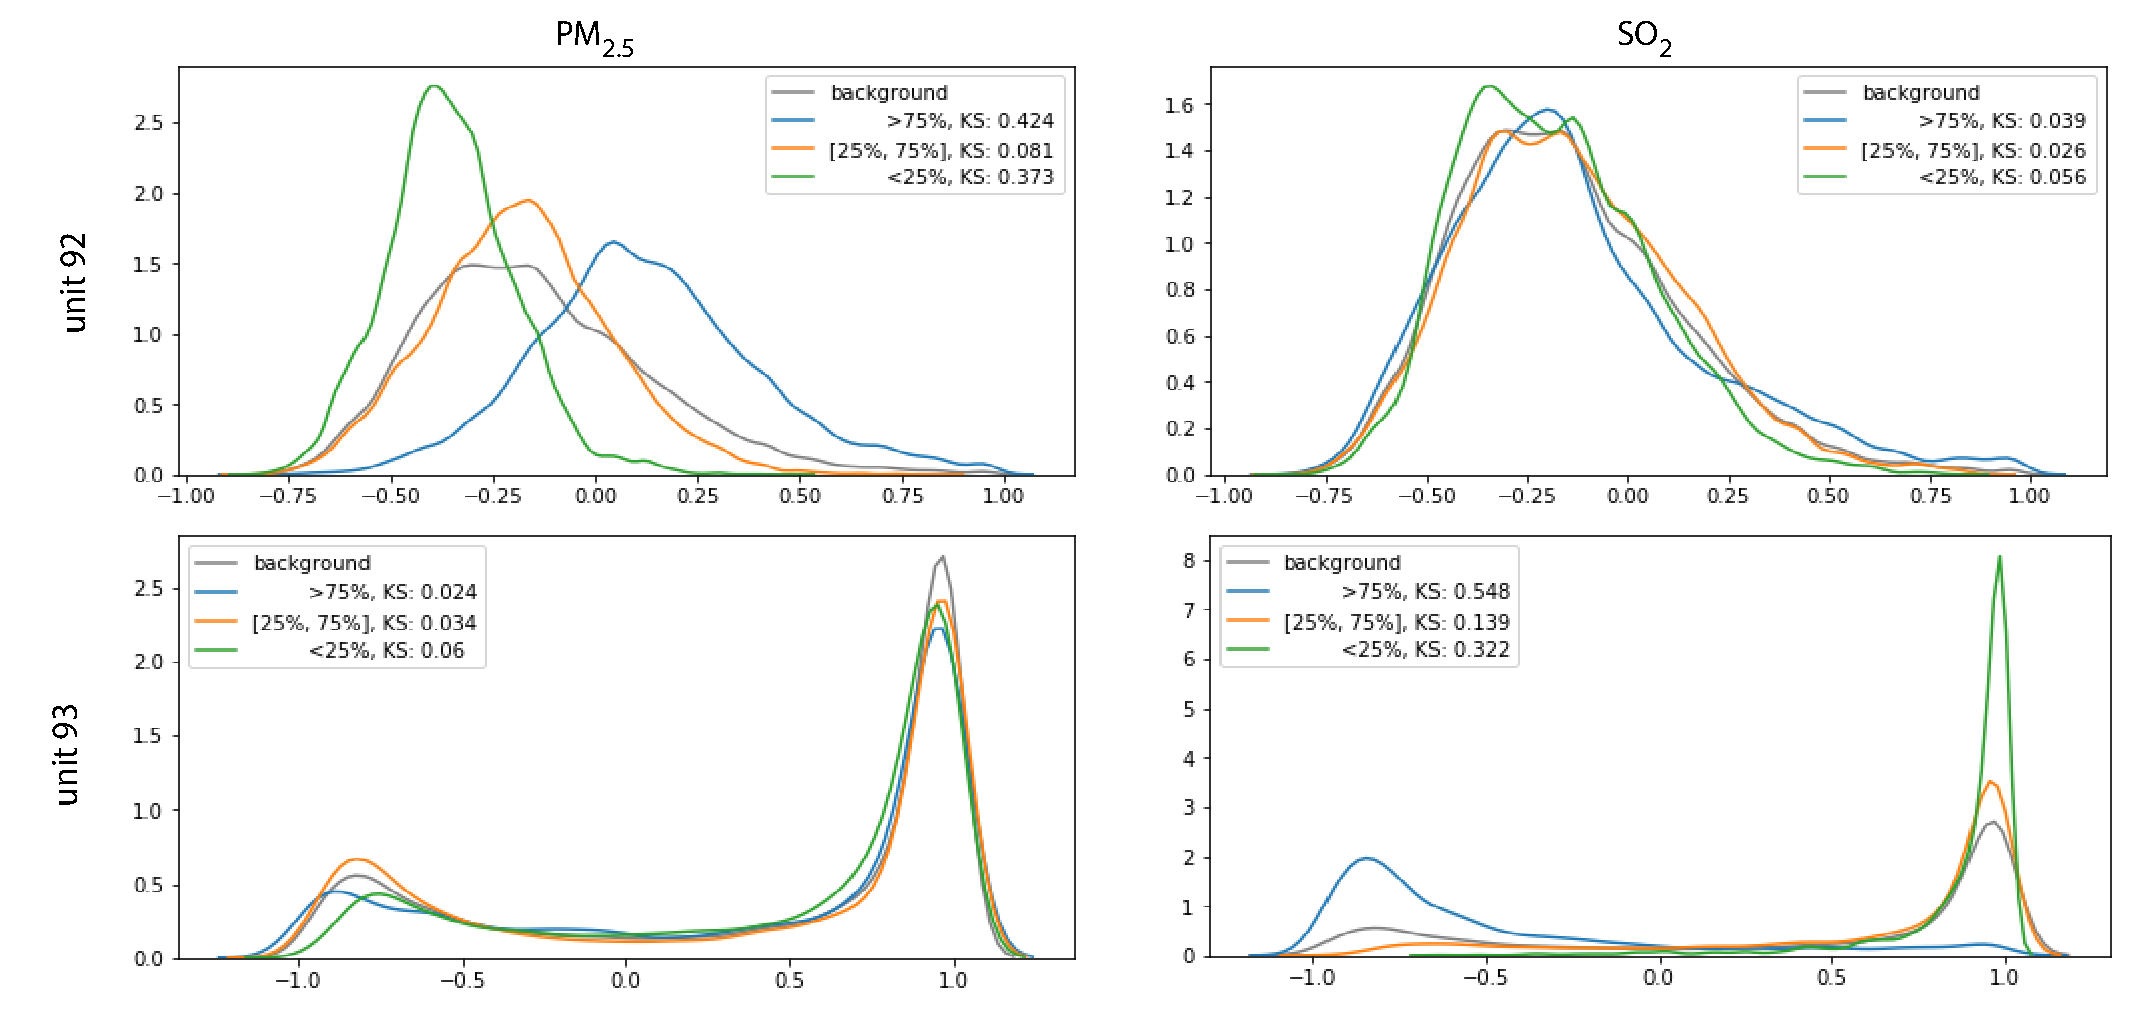
\includegraphics[width=0.45\textwidth]{pictures/methods/unit_response_kdeplot.pdf}
	\vspace{-3mm}
	\caption{Compare the response of hidden units(92 and 93) to features ($PM_{2.5}$ and $SO_2$). 
% 	Top left and bottom right: the distribution of the background is different from the distribution of other feature selections, which shows the hidden unit 92 and 93 response to $PM_{2.5}$ and $SO_2$ respectively.
	}
	\label{fig:unit_distribution_subgroup}
	\vspace{-4mm}
\end{figure}


To quantitatively measure the relationship strength between a hidden unit and a specific input feature, we compare the hidden unit distribution of data in different feature ranges with the distribution of all the data.
A larger difference indicates a stronger relationship as the hidden unit will generate different values when the feature value changes.
Specifically, the relationship strength between the $j^{th}$ hidden unit and feature $f$ can be calculated as:

\begin{equation}
    \label{equation:qualify_response}
    \begin{split}
    RS(j, f) = & max(Dis(\mathsf{H}^{j, f},~\mathsf{H}_{perc<0.25}^{j, f}), \\ 
    & Dis(\mathsf{H}^{j, f},~\mathsf{H}_{0.25~\leq~perc<0.75}^{j, f}), \\ 
    & Dis(\mathsf{H}^{j, f},~\mathsf{H}_{perc~\geq~0.75}^{j, f}))
    \end{split}
\end{equation}



\subsection{Hidden Unit and Feature Clustering} \label{section:clustering}
Another major challenge for interpreting RNN models on multi-dimensional sequential data is scalability.
RNN models usually contain hundreds to thousands of hidden units for each layer, which makes it ineffective to display the activation distribution of every hidden unit to users.
To address this challenge, previous work on visual interpretation of machine learning models usually use clustering~\cite{ming2017understanding, liu2017towards} or sampling~\cite{pezzotti2018deepeyes} techniques to reduce the number of visual elements displayed.
In this work, we choose clustering methods over sampling since clustering can better preserve the hidden units' response relationship to features. It also provides a good summary of the knowledge that the model learned. 

With the measurement of unit response, we can generate a 2D table with the size of $D \times\ M$, where $D$ and $M$ are the size of hidden units and features respectively. The cell of $j^{th}$ row and $k^{th}$ columns is the response of hidden unit $h^j$ to feature $f^k$: $RS(j,f^k)$. Then we can define the response embedding vector for both features and hidden units. For any feature $f^k$ and hidden unit $j$, the response embedding vectors are $vec_{f^k}= [RS(0, f^k), RS(1, f^k), ..., RS(D-1, r^k)]$ and $vec_{j}= [RS(j, f^0), RS(j, f^1), ..., RS(j, f^{M-1})]$, which are the specific columns and rows respectively. 

To analyze the relationship between hidden units and features, Yao et al.~\cite{ming2017understanding} used a bipartite graph to model the many-to-many relationship and used co-clustering algorithms~\cite{dhillon2001co} to group hidden units and input features simultaneously. We test co-cluster techniques: Spectral Co-clustering(SCoC) as well as other techniques including Agglomerative Clustering(AC) and Spectral Clustering(SC) on our dataset. The clustering methods other than SCoC take response embedding vectors as input to cluster features and hidden units respectively. To rank the performance of different clusters with different cluster numbers, we use the Silhouette Coefficient~\cite{rousseeuw1987silhouettes} to evaluate the quality of the clusters. Silhouette Coefficient ranges from -1 to +1,  with higher values of this coefficient meaning the cluster quality is more appropriate. 


Fig.~\ref{fig:cluster_parameters} shows cluster quality for features (left) and hidden units (right). We found that the Spectral Co-clustering method has a low Silhouette Coefficient score because it keeps creating a one-to-one relationship between the feature cluster and the hidden units cluster. In this case, it can be found that Agglomerative Clustering with cluster number of 12 and K-Means with cluster number of 10 show the best performance for feature and hidden units respectively.
With the Silhouette Coefficient, our system can automatically choose the clustering algorithms and cluster number.
Users can also manually choose different clustering algorithms and change the number of clusters based on their analysis requirement.



\begin{figure}[t]
	\centering
	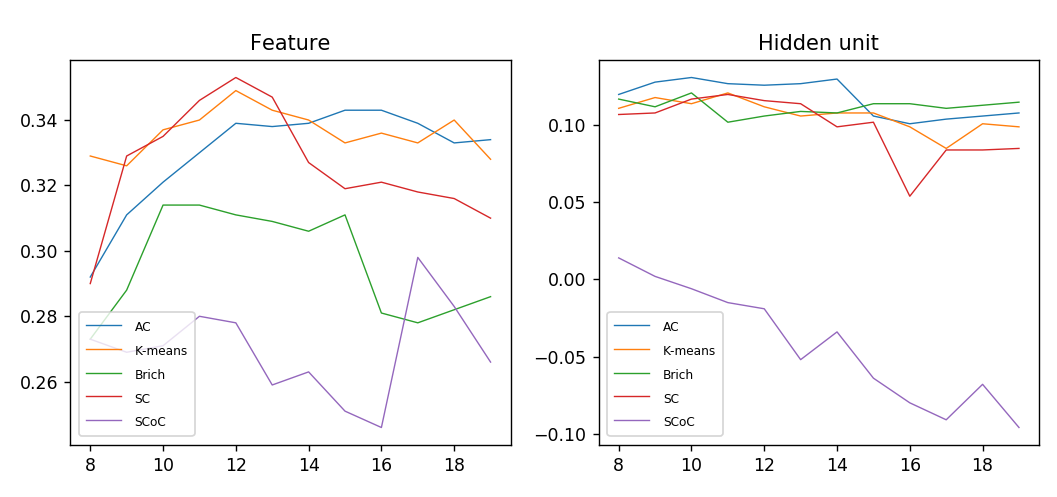
\includegraphics[width=0.45\textwidth]{pictures/methods/cluster_parameters.png}
	\vspace{-3mm}
	\caption{Cluster score with different cluster number. Left: feature cluster. Right: hidden unit cluster. The horizontal axis represents the cluster number, the vertical axis represents the cluster score. 
% 	A good choice of the cluster method and cluster number is K-means and 12 for the feature cluster, Agglomerative Clustering (AC) and 10 for the hidden units cluster.
	}
	\label{fig:cluster_parameters}
	\vspace{-4mm}
\end{figure}

The clustering results can be modeled as bipartite graph $\mathbb{G} = (\mathbb{V}_H, \mathbb{V}_F, \mathbb{E})$, where $\mathbb{V}_H$ is the hidden unit cluster set and $\mathbb{V}_F$ is the feature cluster set. $\mathbb{E}$ indicates the weighted edge set between unit clusters and input dimension clusters with the weight of $E_{H,F} = \displaystyle\sum_{h \in H}\displaystyle\sum_{f \in F}RS(h, f)$ where $H \in \mathbb{V}_H$ and $F \in \mathbb{V}_F$. 

This bipartite graph of features and hidden units can help users understand the information captured by different hidden unit clusters by examining which feature clusters have strong relationships with them.



\subsection{Local Feature Importance}\label{section:feature_importance}

Inspired by back-propagation in machine learning, we conduct the individual level analysis based on the local gradient which is used to present the word saliency in NLP tasks~\cite{li2015visualizing}. 
Given the output of feature $y^l$, we use the local gradient with respect to feature $x_t^k \in x$ to present the feature importance as:

\begin{equation}
    \label{equation:feature_gradient}
    \begin{multlined}
    w(y^l, x_t^k) = |\frac{\partial(y^l)}{\partial(x_t^k)}|
    \end{multlined}
\end{equation}


The absolute value of gradient $w(y^l, x_t^k)$ indicates the sensitiveness of $x_t^k$ to the final decision of  $y^l$ with the given input sequence of $x$. This measurement shows how much the specific feature at a specific time contributes to the final output~\cite{li2015visualizing}.
However, for input $x$ with the length of $T$,  the total number of all feature importance scores is $N \times T$ which causes difficulty in showing the overview. To address this challenge, we leverage the clustering result from Sec.\ref{section:clustering} and define the cluster importance of features as:
\begin{equation}
    \label{equation:cluster_gradient}
    \begin{multlined}
    W(y^l, H^i_t) =\displaystyle\sum_{x^k_t \in H^i_t}|w(y^l, x^k_t)|
 \end{multlined}
\end{equation}
\QM{Thus, the size of the cluster importance for all timestamps is $C \times T$ where $C$ is the number of clusters and $C<N$}. 
